\documentclass[a4paper, 12pt]{article}
\usepackage{parskip}
\usepackage[utf8]{inputenc} 
\usepackage[english]{babel}
\usepackage[letterpaper,top=2cm,bottom=2cm,left=3cm,right=3cm,marginparwidth=1.75cm]{geometry}
\usepackage{biblatex}
\addbibresource{reports/paper/refs.bib}
\usepackage{amsmath}
\usepackage{graphicx}


\title{\textbf{Which of the G10 Currencies is the Riskiest to Hold for a Swiss Resident?}}
\author{Xiao Chen 21-742-820, Yannic Laube, Bosko Todorovic, Zhi Wang}
\date{\today}

\begin{document}
\maketitle
\section{Introduction}
The rapid development of international trade and cross-border investment has promoted the foreign exchange (FX) market to be an increasingly critical component of the global economy. In international trade, the FX market not only provides the basis for currency exchange but also influences the pricing of goods, trade costs, and the competitiveness of businesses. However, uncertainties of exchange rate fluctuations have introduced significant risks and challenges to both international trade and investment~\cite{AUBOIN_RUTA_2013}~\cite{riker2020review}.

According to the Bank for International Settlements (BIS)~\cite{bis2022report}, the daily trading volume of the global FX market has exceeded \$7 trillion, with G10 currencies forming the core of this market due to their high liquidity and active trading. The G10 currencies refer to the group of ten most heavily traded and liquid currencies in the global foreign exchange market. These include the US dollar (USD), euro (EUR), Japanese yen (JPY), British pound (GBP), Swiss franc (CHF), Canadian dollar (CAD), Australian dollar (AUD), New Zealand dollar (NZD), Swedish krona (SEK), and Norwegian krone (NOK). For an open economy like Switzerland, Swiss residents holding assets denominated in other G10 currencies still face potential risks arising from exchange rate fluctuations, such as asset value depreciation, increased transaction costs, and financial market volatility affecting their investment portfolios. Moreover, G10 currencies also play a critical role in various aspects of Swiss residents' financial activities. In this context, analyzing exchange rate fluctuations and evaluating the risk characteristics of G10 currencies from perspective of a Swiss resident carries significant theoretical and practical importance.

This study aims to address the following key question: 'Which of the G10 currencies is the riskiest for Swiss residents?' By utilizing historical data and Monte Carlo simulation methods, this paper evaluates the volatility, Value-at-Risk (VaR), and Expected Shortfall (ES) of each G10 currency to identify the most risky assets. The findings are expected to provide a scientific basis of investment and risk management strategies for Swiss residents.

\section{Literature Review}
A review of the existing literature provides insights into the relationship between exchange rate fluctuations, international trade, and cross-border investments. Auboin and Ruta~\cite{AUBOIN_RUTA_2013} highlight that exchange rate volatility introduces uncertainties for exporters and importers while profoundly impacting cross-border investments. Companies experiencing sharp exchange rate fluctuations may experience revenue shrinkage due to foreign currency depreciation or asset devaluation.

Riker and Wickramarachi~\cite{riker2020review} further argue that persistent exchange rate changes influence multinational corporations' strategic decisions, including investment location choices and capital allocation. For instance, Avdjiev \textit{et al.}~\cite{dollar_exchange} indicate that U.S. dollar appreciation often reduces USD-denominated cross-border banking flows, thereby imposing greater financing and investment risks on countries and corporations heavily reliant on USD debt.

Researches also highlight the role of G10 currencies in the daily activities and investment strategies of Swiss residents. As a key currency in the Euro Area, the euro plays a significant role for Swiss residents in daily financial activities~\cite{engel2016exchange}~\cite{goulferni2023switzerland}. Due to Switzerland's geographical proximity to the Euro Area, EUR is commonly used alongside the Swiss franc for cross-border shopping, travel, and international payments~\cite{sif_imf_reports}. Additionally, high-liquidity G10 currencies such as the US dollar, the euro, and Japanese yen provide Swiss residents with easy access to global investment opportunities, including equities, bonds, and real estate~\cite{rogoff2000six}. Their stability helps reduce exchange rate risks~\cite{campbell2002strategic}~\cite{engel2016exchange}, ensuring more predictable investment returns and mitigating the likelihood of extreme financial losses~\cite{de1998big}. Furthermore, the liquidity and stability of G10 currencies allow Swiss residents to diversify their assets beyond the Swiss franc, a factor particularly relevant during periods of economic uncertainty~\cite{ito2020currency}. Some G10 currencies, such as the Swiss Franc and Japanese Yen, exhibit strong safe-haven properties~\cite{ranaldo2010safe}, enabling Swiss residents to preserve their wealth during periods of global financial turbulence or geopolitical instability. As a globally recognized safe-haven currency, volatility of Swiss Franc in relation to other G10 currencies is important to Swiss residents.

In addition, existing research suggests that FX market risks are often assessed through indicators such as volatility, Value-at-Risk (VaR), and Expected Shortfall (ES)~\cite{AUBOIN_RUTA_2013}~\cite{dollar_exchange}~\cite{riker2020review}. Monte Carlo simulation methods are also frequently employed to forecast future price paths, assisting investors in identifying potential extreme risks.

However, systematic comparisons of G10 currency risks from the perspective of Swiss residents are scarce in the existing literature. This report aims to address this gap by evaluating the risk characteristics of G10 currencies through historical data analysis and simulation-based methods.

\section{Methodology}

Various quantitative approaches were applied in this study to assess the exchange rate risk of the G10 currencies against the Swiss Franc. The methods used include the calculation of Value-at-Risk (VaR) through different models, the analysis of volatilities, and the investigation of the sensitivity of exchange rate returns to interest rate differentials. These approaches are described in detail in the following subsections.

\subsection{Calculation of Value-at-Risk (VaR)}

Value-at-Risk (VaR) indicates the loss that will not be exceeded with a certain probability and within a specified time period. In this analysis, a holding period of one day was chosen, and a confidence level of 95\% was used. Two different methods for calculating VaR were applied: the historical calculation and the Monte Carlo simulation for a forward-looking VaR calculation.

The historical calculation is based on the empirical distribution of historical returns. The daily exchange rate return was calculated for each currency, and the 5\% quantile of the distribution was used as the estimate for VaR. This method does not make any assumptions about the distribution of returns and thus reflects realistic market conditions.

As part of the Monte Carlo simulation for the value-at-risk (VaR) of exchange rates, 10 simulations were conducted to examine possible future scenarios for the exchange rate development of the G10 currencies against the Swiss franc (CHF). The Value-at-Risk (VaR) for the simulated price paths and simulated returns was calculated for the last period of the simulation, and the VaR was explicitly visualized in the return simulation.
First, simulated price paths for each currency were generated. These price paths were simulated using the most recent prices and daily volatility, and then visualized, without explicitly displaying the VaR.
In a subsequent step, simulated returns were calculated based on the generated price movements. These returns were visualized over the simulated periods to represent the fluctuation range of the returns. The VaR 5\% for the simulated returns was explicitly calculated for the last day of the simulation and displayed as a horizontal line in the charts. This line marks the maximum loss that will not be exceeded with 95\% probability.

\subsection{Volatility Analysis}

Volatility was calculated as a measure of the fluctuation intensity of the exchange rates. It was determined based on the standard deviation of the daily returns. High volatility values indicate increased risk, as larger fluctuations in exchange rates imply higher uncertainties. The volatilities of the G10 currencies were compared to identify which currency poses the greatest risk for a Swiss investor. Additionally, time series plots were created to visualize volatility trends during the study period.

\subsection{Regression to Analyze Interest Rate Differentials}

The sensitivity of exchange rate returns to interest rate differentials was examined using linear regression analysis. For each currency, a model was estimated where the logarithmic exchange rate return (\(\text{log\_return}_{\text{exchange}}\)) was the dependent variable, and the difference in logarithmic interest rates (\(\text{log\_diff}_{\text{interest\_rate}}\)) was the independent variable:

\[
\text{log\_return}_{\text{exchange}} = \alpha + \beta \cdot \text{log\_diff}_{\text{interest\_rate}} + \epsilon
\]

The regression analysis determined the parameters \(\alpha\) (intercept) and \(\beta\) (sensitivity of returns to interest rate differentials). Significance tests and confidence intervals were used to assess the statistical significance of the parameters. A detailed summary of the regression was created for each currency.

\section{Data}
\section{Results}

\section{Conclusion}
\section*{Appendix}
\begin{figure}[h]
    \centering  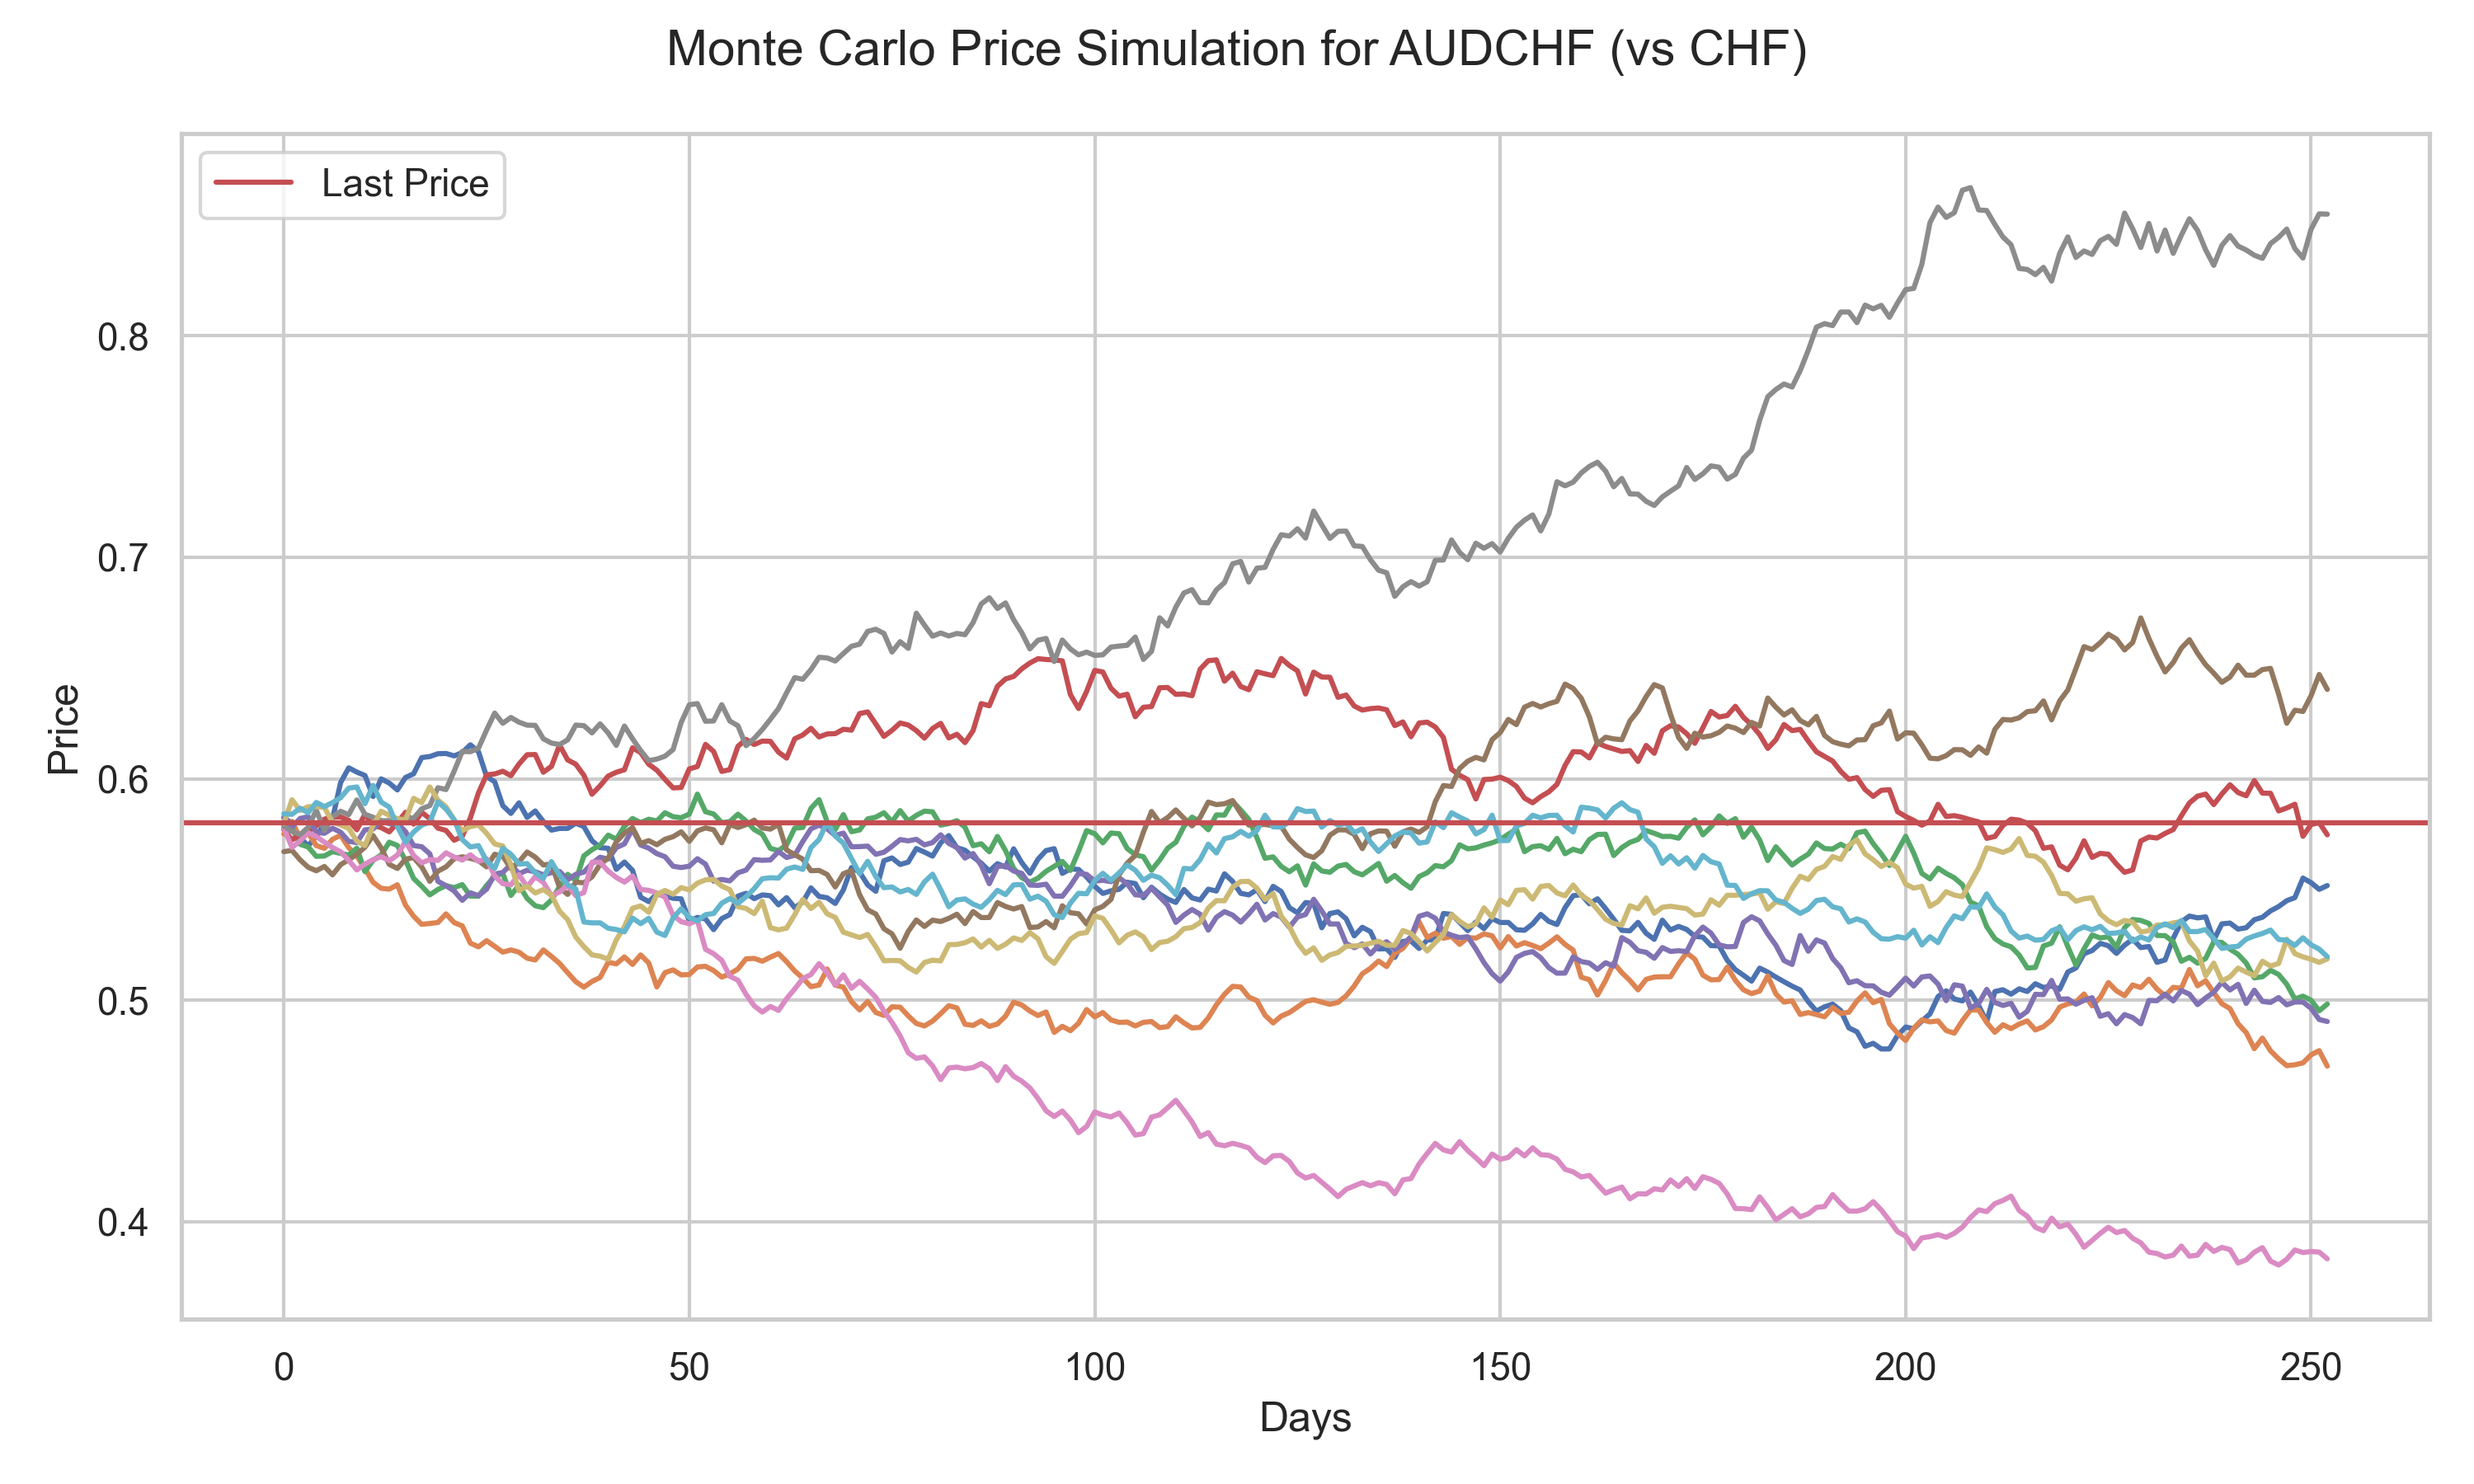
\includegraphics[width=0.8\linewidth]{reports/figures/monte_carlo_price_simulation_AUDCHF_vs_CHF.png}  \label{fig:monte_carlo_price_simulation_AUDCHF_vs_CHF}
    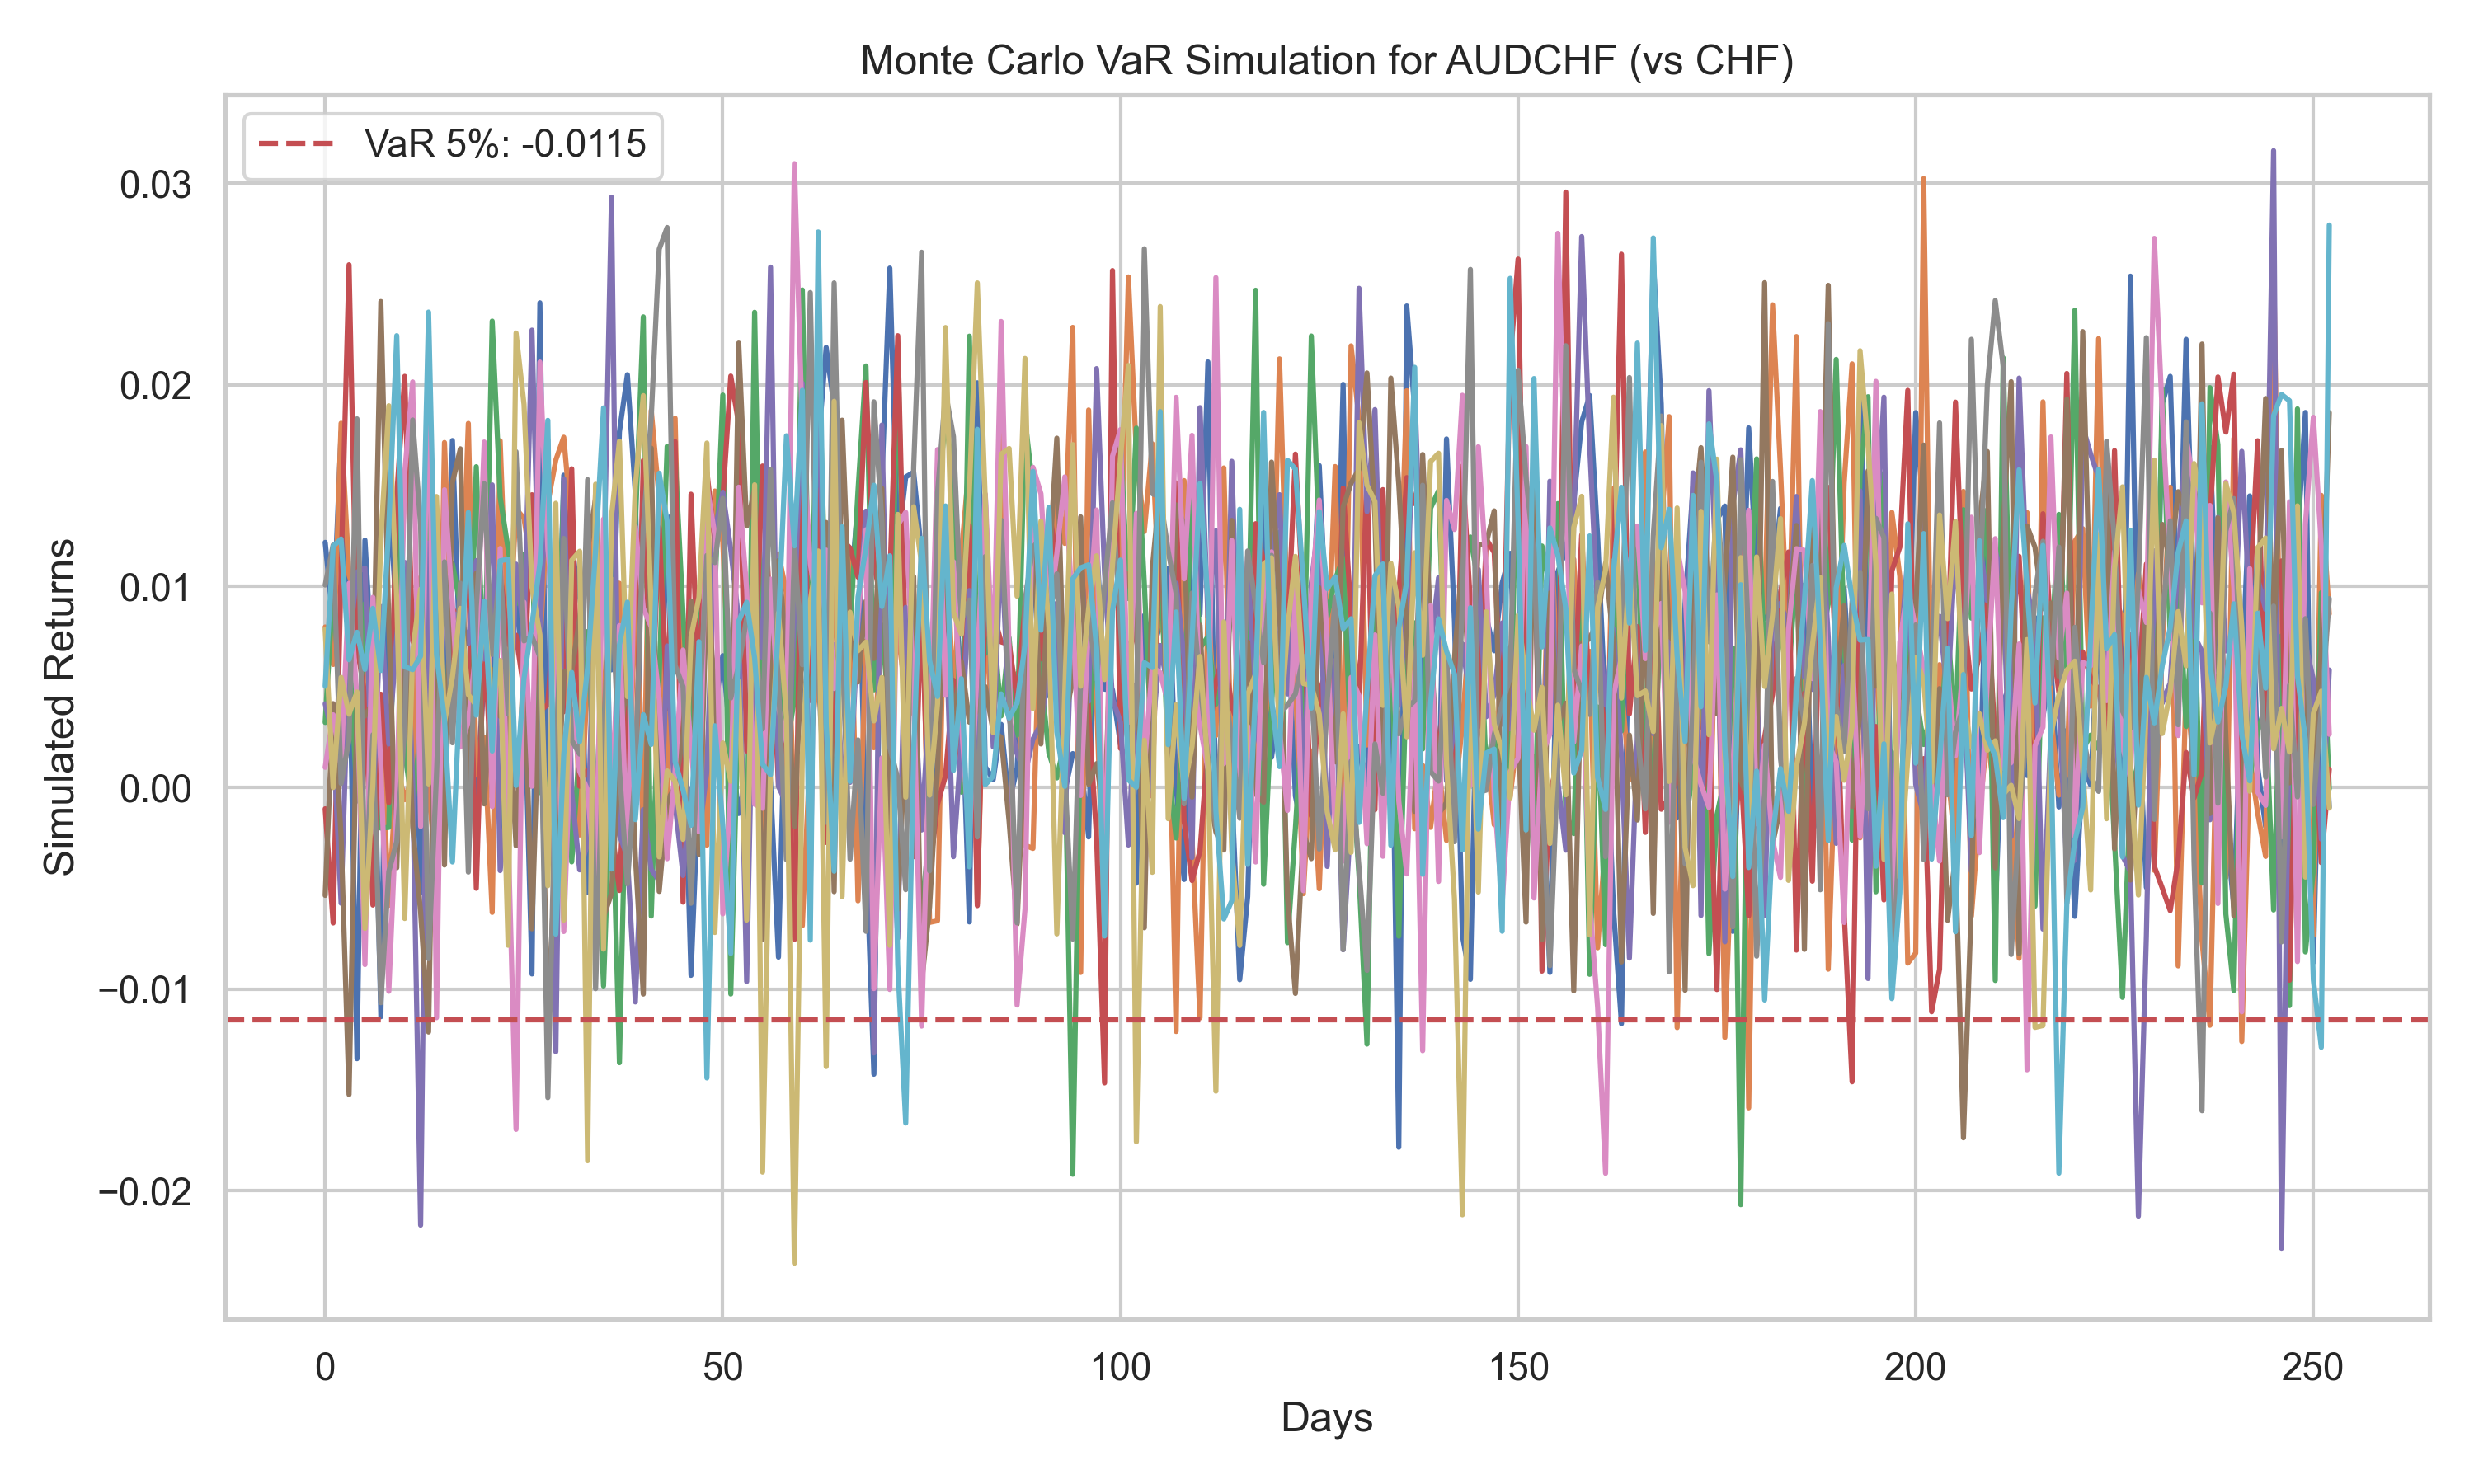
\includegraphics[width=0.8\linewidth]{reports/figures/monte_carlo_var_simulation_AUDCHF_vs_CHF.png}  \label{fig:monte_carlo_var_simulation_AUDCHF_vs_CHF}
    \caption{\footnotesize Monte Carlo price siulation (left) and VaR simulation (right) for AUD-CHF.}
\end{figure}
\begin{figure}
    \centering  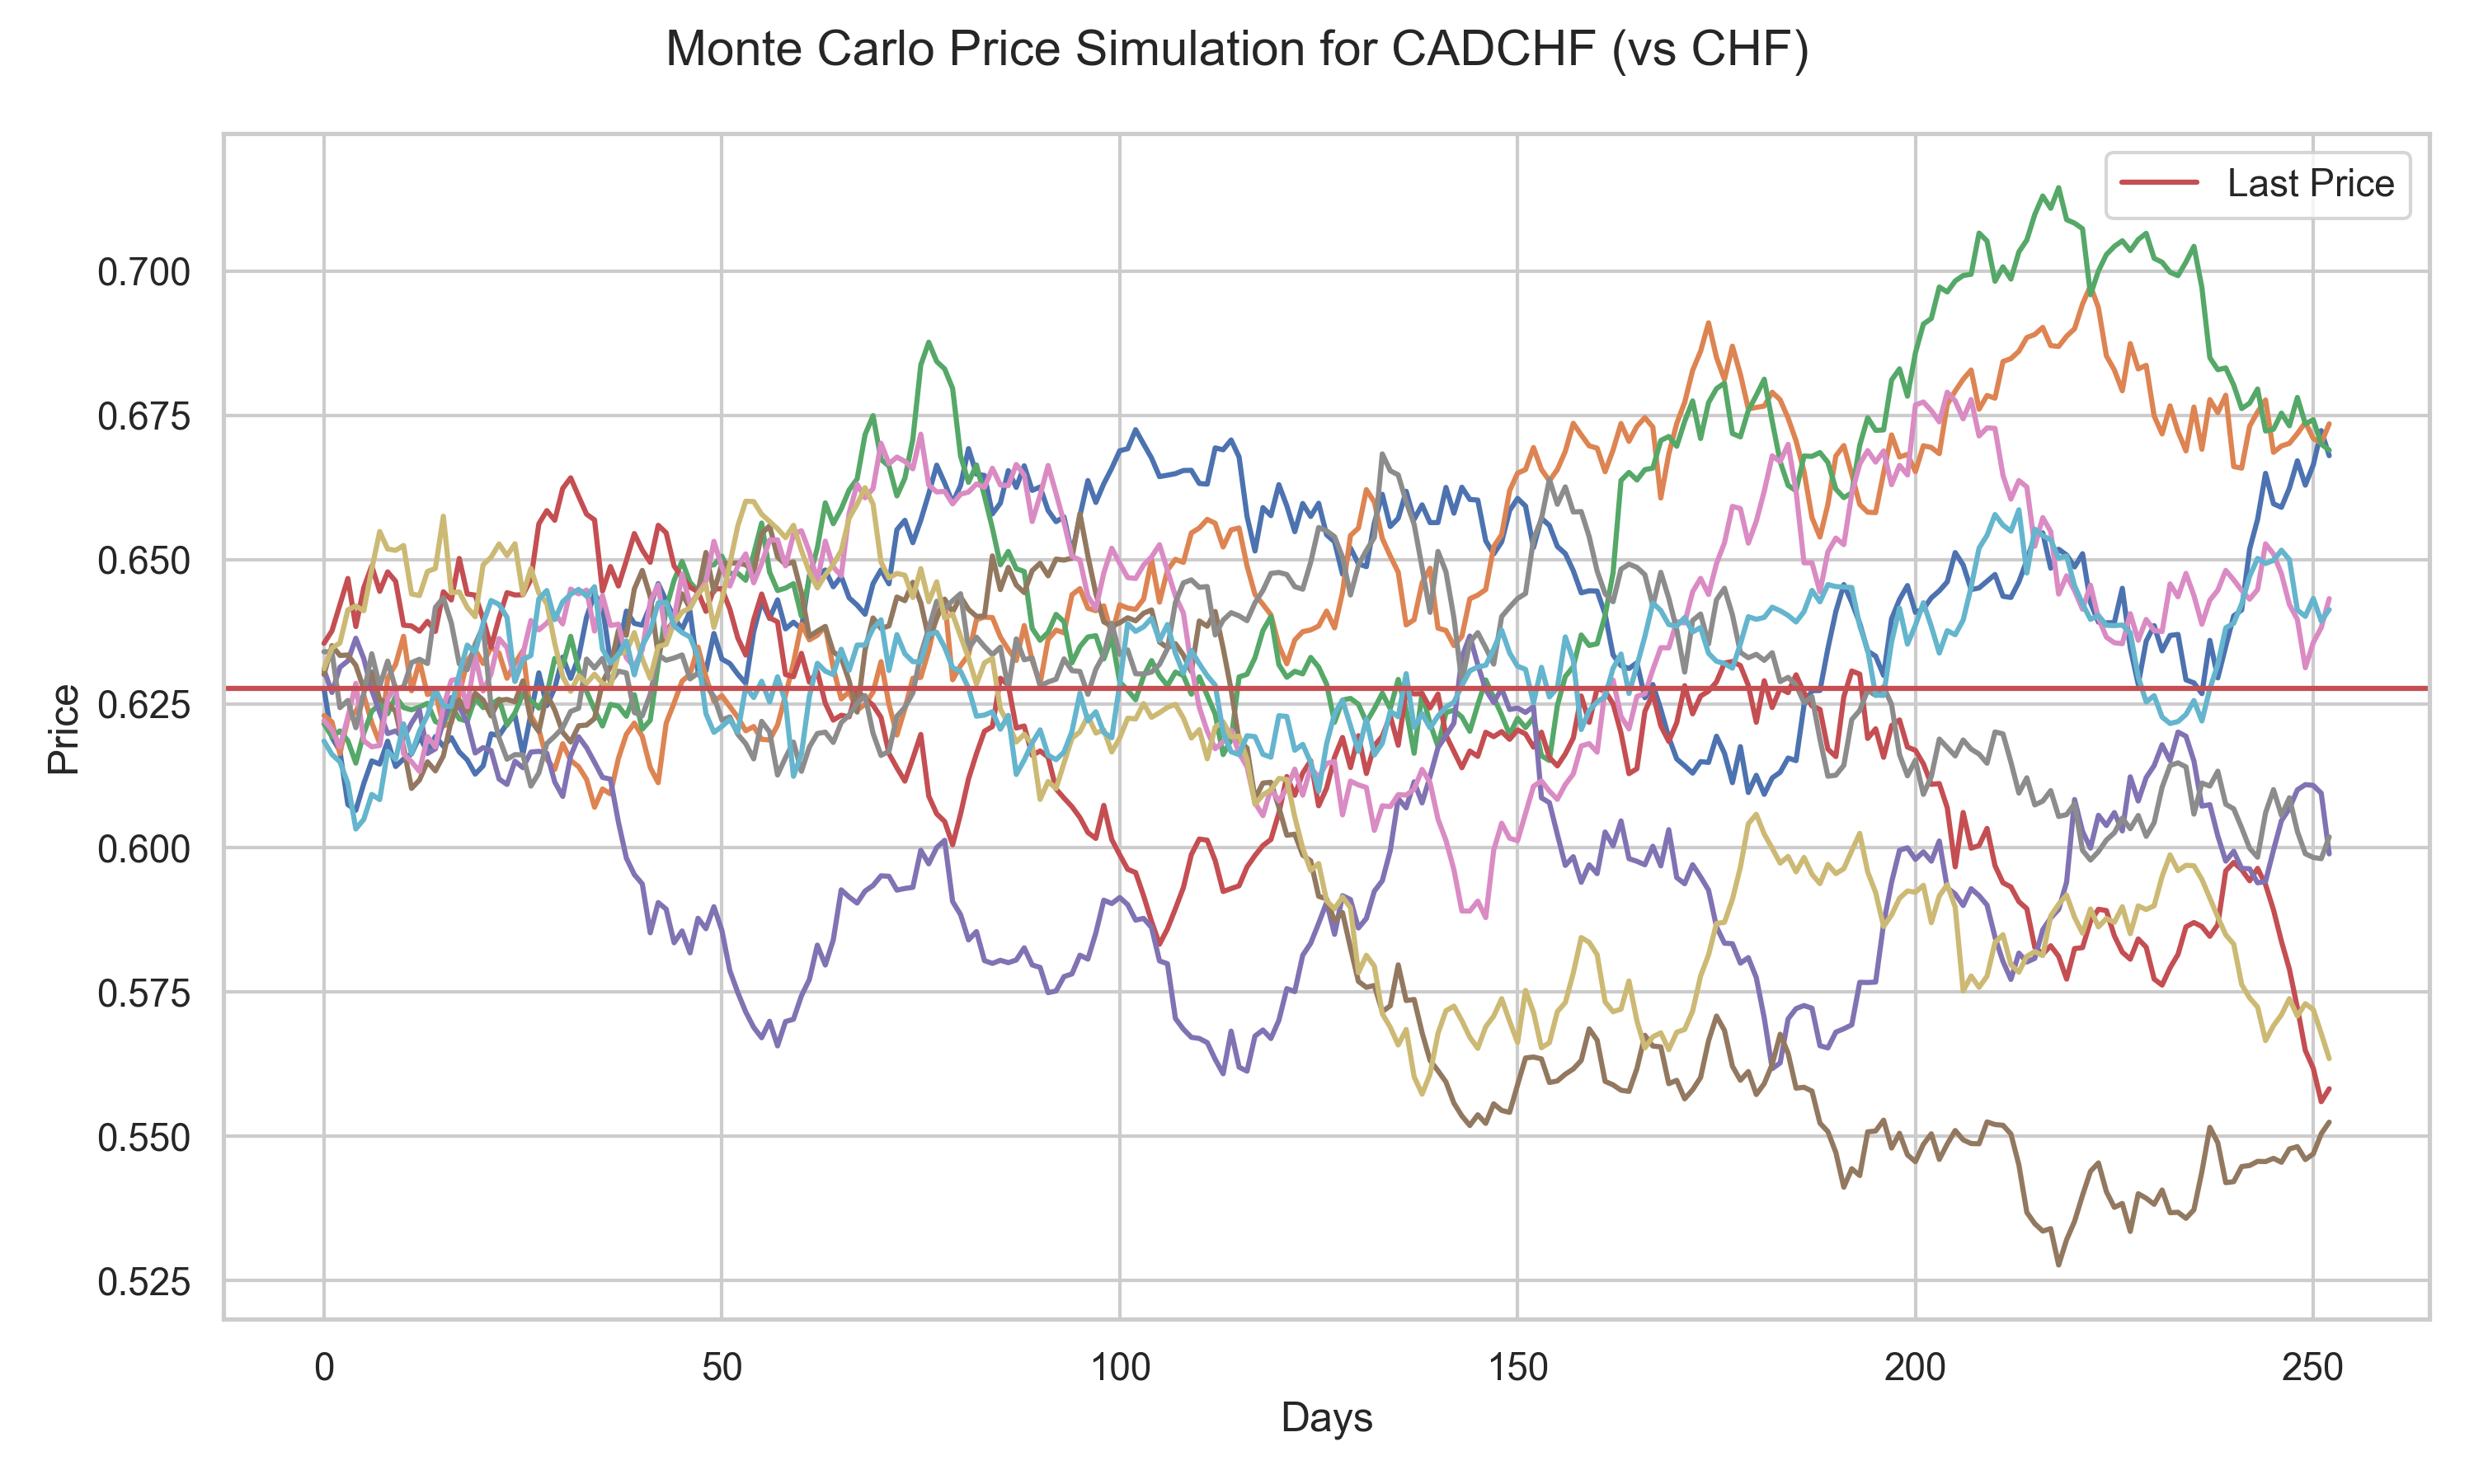
\includegraphics[width=0.48\linewidth]{reports/figures/monte_carlo_price_simulation_CADCHF_vs_CHF.png} \label{fig:monte_carlo_price_simulation_CADCHF_vs_CHF}
    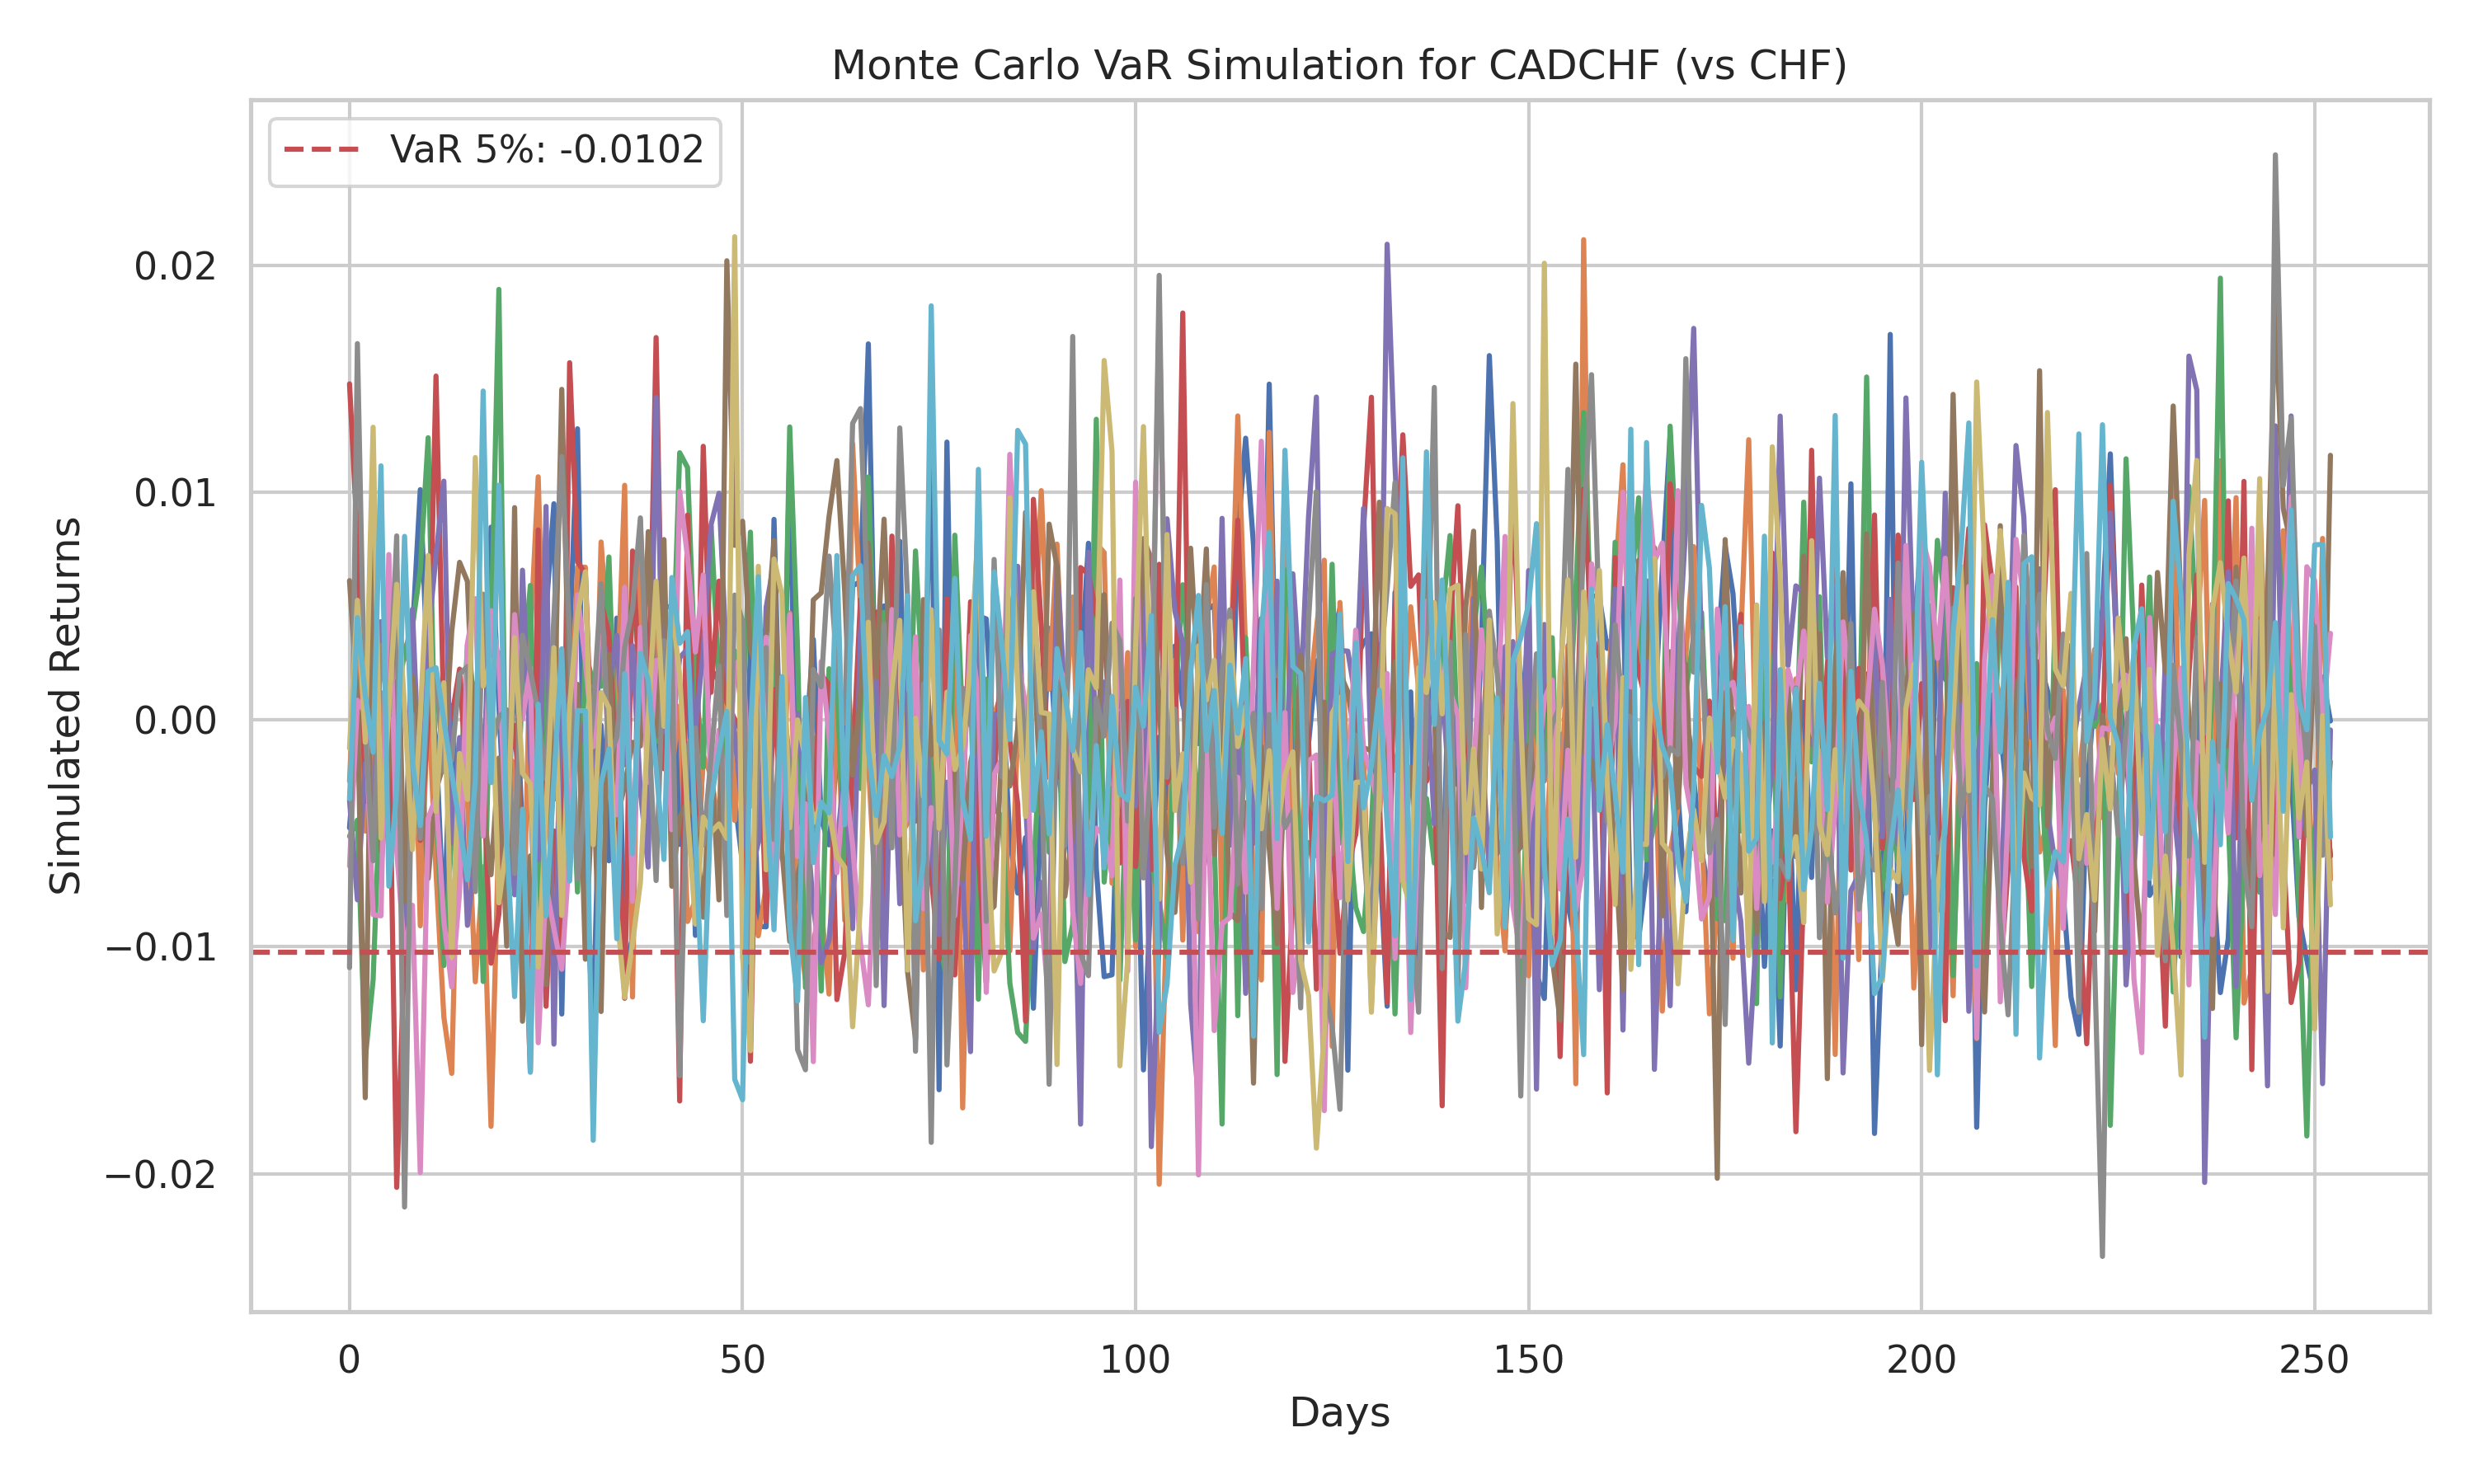
\includegraphics[width=0.48\linewidth]{reports/figures/monte_carlo_var_simulation_CADCHF_vs_CHF.png} \label{fig:monte_carlo_var_simulation_CADCHF_vs_CHF}
    \caption{\footnotesize Monte Carlo price siulation (left) and VaR simulation (right) for CAD-CHF.}
\end{figure}
\printbibliography
\end{document}